\section[Matched Pulses \& Simultons]
    {Matched Pulses \& Simultons in Three-Level Atoms}
  \label{sec:nonlinear_simultons}

      The study of optical solitons propagating due to self-induced
      transparency, summarised in section \ref{sec:sit}, can be extended to
      consider short resonant pulses in three-level media. It has been
      determined theoretically that simultaneous optical solitons --- or
      \textit{simultons} --- propagating at the different transition wavelengths
      exist as analytic solutions to the three-level \textsc{mb} equations.

  \subsection{Literature Review}

    As the results of this work on short resonant pulses in three-level atoms,
    beginning in the 1980s, are less familiar than that of soliton propagation
    in the two-level system, we take the opportunity here to review some of the
    key developments.

    The first studies on propagation of simultaneous, different-wavelength
    optical pulses were made by Konopnicki \& Eberly,
    1981\cite{Konopnicki1981,Konopnicki1981a}. The authors derived analytic
    solutions to the \textsc{mb} equations representing optical solitons
    propagating simultaneously at different wavelengths, which they named
    \textit{simultons}. They found analytic descriptions for exactly matched
    sech pulses with identical oscillator strengths (\ie $g_{01} = g_{02}$ in
    the \textsc{mb} model) in $\Xi$-type and $V$-type three-level media.

    Further analytic work by Kujawski, 1982\cite{Kujawski1982} showed that the
    \textsc{mb} equations for the three-level system on two-photon resonance can
    be reduced to the sine-Gordon equation\cite{lamb1980elements}, thus
    confirming that the simulton is an optical soliton solution. The author also
    showed that the conditions required for multi-simulton propagating are the
    same as Konopnicki \& Eberly showed for single simultons.

    Eberly, 1999 looked at transmission of dressed fields in $\Lambda$-type
    three-level media\cite{Eberly1999}. The $\Lambda$ system has a dark state
    which is able to trap population (we will consider this further in chapter
    \ref{chp:polaritons}). The analytic solution in this case showed that the
    probe envelope $\Omega_p$ is of the familiar sech shape while the coupling
    envelope must be of a tanh profile, in a counter-intuitive pulse sequence
    similar to that employed in \textsc{stirap}.

    Rahman \& Eberly, 1998, provided\cite{Rahman1998} an ansatz for analytic
    solution of the three-level MB equations for Doppler-broadened pulse pairs,
    including analytic solutions for pulse amplitude, excited state population,
    group and phase velocities. In an associated numerical study, the same
    authors looked at\cite{Rahman1999} propagation of pulses in V-type media
    with inhomogeneous broadening. The authors relaxed the conditions imposed by
    the analytic model to include non-matched pulses and non-sech envelopes,
    finding that it is possible for non-matched pulses to match themselves in
    certain conditions and that, as in the two-level case, the sech shape is a
    natural steady state for V-type pulses rather than a mathematically singular
    solution, and so other pulse envelopes will propagate. Finally, they
    demonstrated the numerical validity of a two-photon pulse area theorem,
    including the case of pulse breakup.

  \subsection{The Two-Photon Area Theorem}

    We will consider the V-type system similar to that described in the latter
    papers by Rahman and Eberly\cite{Rahman1999}, and present some numerical
    results from our \textsc{mb} model for this system. We start with a
    quantised V-type three-level atom as illustrated in figure
    \ref{fig:three_level_diagrams}.

    The total electric field vector for the two laser beams is described by
    \begin{equation}\label{eqn:env_carrier}
      \mathbf{E}(z,t) = \left[ \tfrac{1}{2} \mathbf{\hat{x}}_p 
        \mathcal{E}_p(z,t) \ee^{\ii(k_p z - \omega_p t)} + 
        \tfrac{1}{2} \mathbf{\hat{x}}_c \mathcal{E}_c(z,t) \ee^{\ii(k_c z -
        \omega_c t)} + \cc \right]
    \end{equation}
    where $\mathbf{\hat{x}}_p$ and $\mathbf{\hat{x}}_c$ are orthogonal
    polarisations of the fields and the envelopes $\mathcal{E}_p$ and
    $\mathcal{E}_c$ are in general complex functions. We define corresponding
    Rabi frequencies $\Omega_p = d_{01}\mathcal{E}_p/\hbar$ and $\Omega_c =
    d_{02}\mathcal{E}_c/\hbar$ where $d_{0j}$ is the dipole moment between level
    $\Ket{0}$ and $\Ket{j}$, which we take parallel to its respective field
    polarisation.

    The Hamiltonian for the V-type three-level atom interacting with these two 
    classical fields is
    \begin{equation}\label{eqn:vee_hamiltonian}
      \mathcal{H}_\mathrm{V} = -\hbar (\Delta_p \sigma_{11} + \Delta_c 
      \sigma_{22}) -\frac{\hbar}{2} 
      \left[ (\Omega_p \sigma_{10} + \Omega_c \sigma_{20} )
      + \hc \right]
    \end{equation}
    within the dipole approximation and in the frame rotating with the
    frequencies of the optical fields. Here $\sigma_{ij} := \Ket{i}\Bra{j}$ is
    the transition operator. The detunings of the fields are represented by
    $\Delta_p$ and $\Delta_c$.

    We may imagine a pair of synchronised input fields, such that
    \begin{equation}
      \Omega_c(0, \tau) = r \Omega_p(0, \tau)
      \label{eqn:matched_fields}
    \end{equation}
    for some constant $r$. The labels $p$ and $c$ denote the typical probe-
    coupling setup in three-level atom experiments. It can be
    shown\cite{Rahman1998} by substitution into the \textsc{mb} equations that
    the system is equivalent to the two-level system addressed by a single
    pulsed field.

    The concept of the area theorem then extends to the pair of field envelopes
    with
    \begin{equation}
      \theta(z) = \sqrt{\theta_c(z)^2 + \theta_p(z)^2}
      \label{fig:vee_area}
      \end{equation}

    where $\theta_c(z)$ and $\theta_p(z)$ are the areas of the coupling and
    probe pulses defined in the same way as equation (\ref{eqn:pulse_area}). A
    pair of pulses that can be expressed in the form of equation
    (\ref{eqn:matched_fields}) are known as \textit{matched pulses}.

    Equation (\ref{fig:vee_area}) does not constrain the individual pulse areas,
    and so predicts that matched pulses will propagate through the medium even
    if the area of either or both of the individual pulses would not be strong
    enough to support a soliton solution in a two level system.

    \begin{figure}[h]
      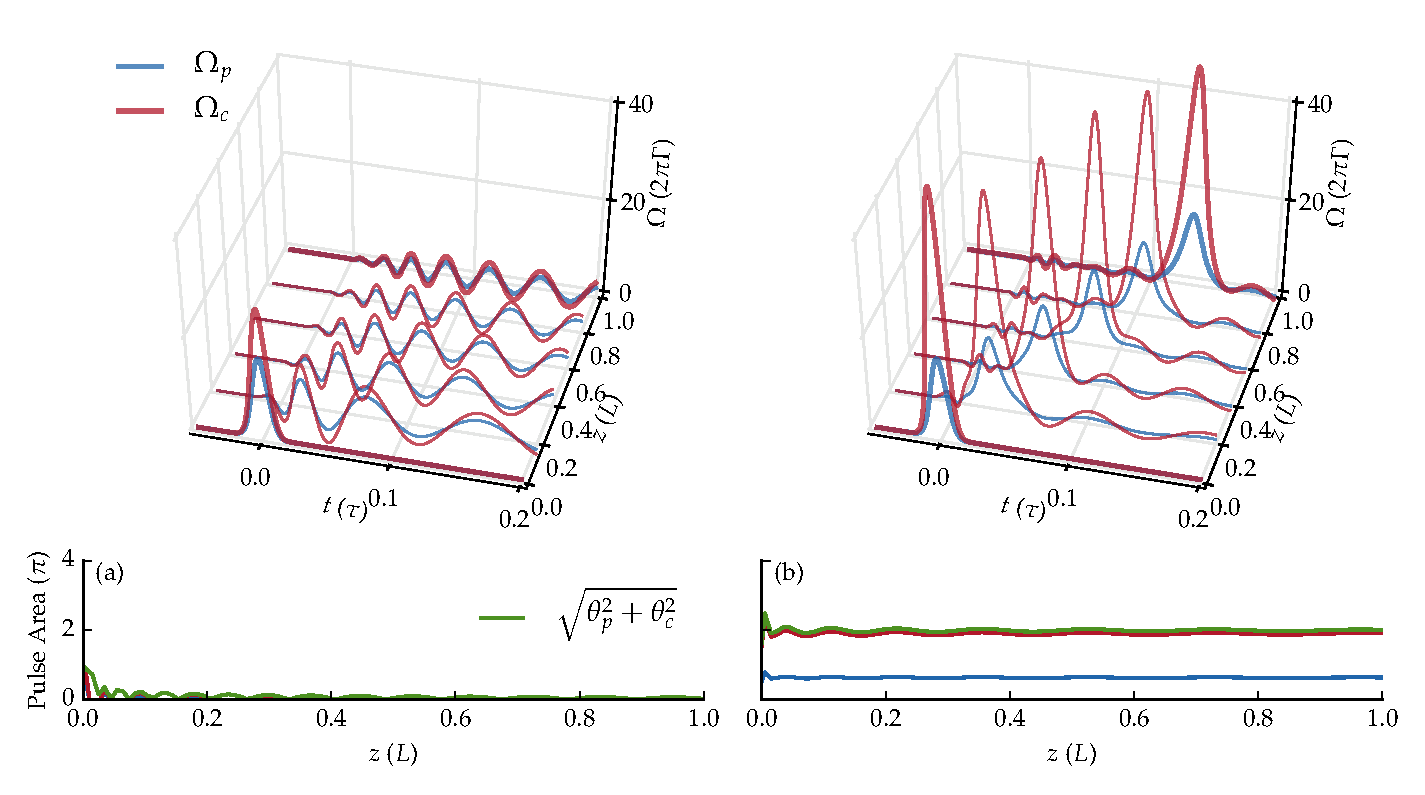
\includegraphics[width=\linewidth]
        {figs/03_nonlinear/mb_vee_sit_05pi_plot_nodecay_fig1.pdf}
      \caption{
      Propagation of matched pulses. (a) A probe input $0.5 \pi$ pulse with a
      $0.8 \pi$ coupling pulse. (b) A probe input $0.5 \pi$ pulse with a $1.5
      \pi$ coupling pulse, showing (top) profiles of the real part of the
      complex Rabi frequencies $\Omega(z, \tau)$ and (bottom) pulse areas
      $\theta(z)$.
      }
      \label{fig:vee_simultons}
    \end{figure}    

    In figure \ref{fig:vee_simultons} we show example numerical results for
    propagation of matched pulses in a V-type medium. In both cases the input
    probe pulse has an area $\theta_p = 0.5 \pi$. The medium is specified such
    that $Ng = \unit[2\pi~10^3]{\Gamma/L}$ on both transitions and spontaneous
    decay is neglected. In figure \ref{fig:vee_simultons}(a) the input coupling
    pulse has area $\theta_c = 0.8 \pi$, such that the total area given in
    equation (\ref{fig:vee_area}) is $\theta(z{=}0) = 0.9 \pi$. We see that
    neither of the fields propagates, both are absorbed and $\theta(z)
    \rightarrow 0 \pi$. In figure \ref{fig:vee_simultons}(b), the input
    coupling pulse has area $\theta_c = 1.5 \pi$, such that the total area
    $\theta(z{=}0) = 1.6 \pi$. We see that both fields propagate as sech-type
    solitons such that $\theta(z) \rightarrow 2 \pi$.

    This striking result suggests that it is possible for weaker pulses to
    propagate through media they they would ordinarily find opaque, by virtue of
    them being `carried along' with an exactly matched coupling pulse.

    % [TODO: robustness of pulses, diff abs, decoherence, thermal broadening]